\documentclass[]{article}

\usepackage[T1]{fontenc}
\usepackage[utf8]{inputenc}
\usepackage[french]{babel}
\usepackage[]{graphicx}
\usepackage[]{hyperref}
\usepackage{pdflscape}

\title{Plan de management projet}
\author{
    Responsable\\
    \\
    Julien Wattier\\
    \\
    \\
    Contributeurs\\
    \\
    Théo Delmas\\
    Lauric Teysseyre\\
    Pierre-Louis Renon\\
    \\
    \\
    Approbateurs\\
    \\
    Frédéric MIGEON\\
    Gilles LEPINARD\\
    \\
    \\
    Université Paul Sabatier\\
    Master Informatique 1\\
   } 
\date{}


\begin{document}
\maketitle
\newpage
\tableofcontents
\newpage

{
    \setlength{\parindent}{0pt} %Retire les alinéas
    \begin{section}{\label{sec:Objectif du document}Objectif du document}
     Ce document a pour objectif d'exposer les méthodes de management appliquées à ce projet.

     Il permet également de suivre le statut actuel du projet et référencement différents documents de suivis.
    \end{section}

    \begin{section}{\label{sec:Contexte et objectifs du projet}Contexte et objectifs du projet}
     \begin{subsection}{\label{sec:Context}Contexte}
         FlopEDT! est une application permettant de créer un emploi du temps satisfaisant une série de contraintes basées sur la programmation linéaire. Cependant la gestion actuelle de ces contraintes est relativement technique et peu documentée.

         De plus les principaux collaborateurs du projet ont initié un découplage entre le back-end et le front-end, les deux parties étant actuellement gérées par un unique serveur.
     \end{subsection}

     \begin{subsection}{\label{sec:Objectifs}Objectifs}
         L’objectif est de créer un système permettant de récupérer et d’afficher les documentations relative à des contraintes, le tout respectant le contexte de découplage front/back de l'application.

         Ces demandes sont à l’initiative du principal développeur du projet Pablo SEBAN. Ce projet est donc à façon pour cette même personne.
     \end{subsection}

     \begin{subsection}{\label{sec:Liste des parties prenantes}Liste des parties prenantes}
         Les parties prenantes sont listées ci-dessous ainsi que leurs besoins principaux, leurs représentants, la modalité de validation des besoins et la recette.

         Les utilisateurs finaux et contributeurs seront considérés uniquement au travers du client.

         \begin{subsubsection}{\label{sec:Maître d’ouvrage}Maître d’ouvrage}
             Besoin : Obtenir une interface intuitive pour son produit permettant aux usagers finaux non techniciens de facilement trouver et ajouter des contraintes.

             Représentants : Pablo Seban

             Validation : voir la \hyperref[sec:Validation des besoins]{validation des besoins}

             Recette : voir la \hyperref[sec:Gestion des besoins]{gestion des besoins}
         \end{subsubsection}

         \begin{subsubsection}{\label{sec:Collaborateur du projet}Collaborateur du projet}
             Besoin : Obtenir une nouvelle version du système maintenable.

             Représentants : Pablo Seban

             Validation : voir la \hyperref[sec:Validation des besoins]{validation des besoins}

             Recette : voir la \hyperref[sec:Gestion des besoins]{gestion des besoins}
         \end{subsubsection}

         \begin{subsubsection}{\label{sec:Utilisateur final}Utilisateur final}
             Besoin : Obtenir une nouvelle version du système utilisable avec efficacité.

             Représentants : Pablo Seban

             Validation : voir la \hyperref[sec:Validation des besoins]{validation des besoins}

             Recette : voir la \hyperref[sec:Gestion des besoins]{gestion des besoins}
         \end{subsubsection}

         \begin{subsubsection}{\label{sec:Fournisseur}Fournisseur}
             Besoin : Satisfaire au mieux les demandes du client.
             Monter en compétence.

             Représentants : Théo DELMAS, Lauric TEYSSEYRE, Pierre-Louis RENON, Julien WATTIER.


             Validation : Non concerné.

             Recette : Non concerné.
         \end{subsubsection}

         \begin{subsubsection}{\label{sec:Assistant de maîtrise d’ouvrage}Assistant de maîtrise d’ouvrage}
             Besoin : Répondre aux demandes de soutien de la part du maître d'ouvrage dans la gestion de ce projet.

             Représentants : Léo CUSSEAU, Florian AZIZEN.

             Validation : Non concerné.

             Recette : Non concerné.
         \end{subsubsection}

         \begin{subsubsection}{\label{sec:Professeur}Professeur}
             Besoin : Obtenir des documents de gestion clairs et de qualité.

             Représentants : Frédéric MIGEON, Gilles LEPINARD.

             Validation : Défini lors des cours relatifs à l’UE.

             Recette : Évaluation itérative des documents tous les mois.
         \end{subsubsection}
     \end{subsection}
    \end{section}

    \newpage

    \begin{section}{\label{sec:Référentiel de management de projet}Référentiel de management de projet}
     \begin{subsection}{\label{sec:Product Breakdown Structure}Product Breakdown Structure}
         Le product breakdown structure défini l’ensemble des produits que doit produire ce projet. Pour chaque produit la méthode de réalisation est présentée.

         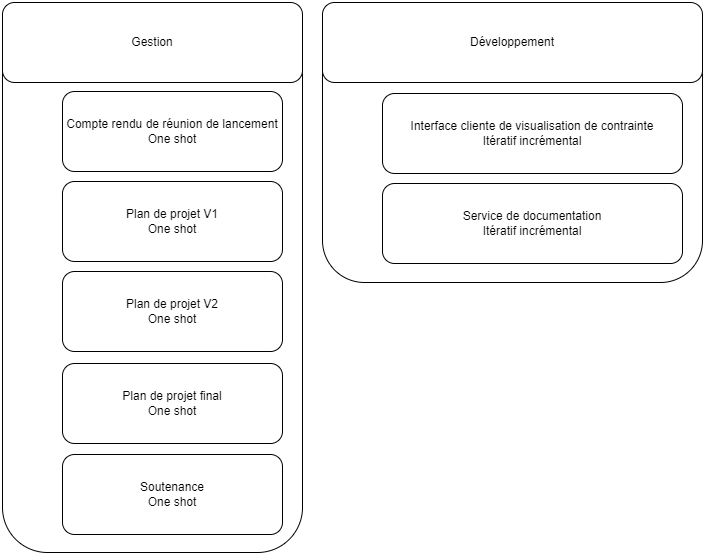
\includegraphics[scale=0.4]{documents/IMG/PBS}
     \end{subsection} 

     \newpage

     \begin{subsection}{\label{sec:Activités du projet}Activités du projet}
         \begin{subsubsection}{\label{sec:Work Breakdown Structure}Work Breakdown Structure}
             Le work breakdown structure défini l’ensemble des activités nécessaires pour réaliser ce projet. Il s’organise en deux parties : La première présente les activités relatives au plan de projet, et la seconde celles au développement, découpées en sprint.

             Ces deux grandes parties seront effectuées en parallèle. Cependant le contenu de ces parties sera effectué de manière séquentielle à cause de leur dépendance. Chaque nœud de la structure précise quelles sont ses entrées et ses sorties.

             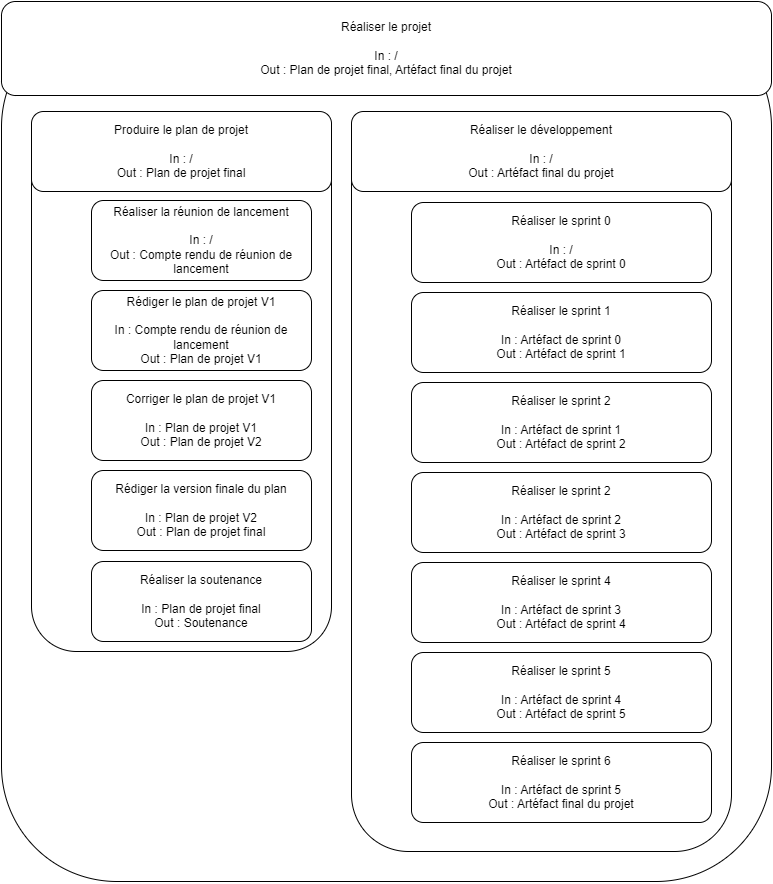
\includegraphics[scale=0.45]{documents/IMG/WBS}
         \end{subsubsection}

         \newpage

         \begin{subsubsection}{\label{sec:Calendrier des ressources}Calendrier des ressources}
             Ce projet est sans ressources matérielles.

             Concernant l’équipe, elle est disponible le jeudi et le vendredi sur la période fixe du 05/01/2023 au 28/04/2023. Les horaires restent souples mais chaque membre devra être disponible au moins 7 heures sur ces deux jours.

             L’équipe sera en congé le 02/03/2023 et le 03/03/2023.

             Il est également possible qu’elle ne soit pas disponible les deux dernières semaines de la période de projet en fonction des examens universitaires.
         \end{subsubsection}

         \begin{subsubsection}{\label{sec:Liste des jalons}Liste des jalons}
             L’équipe effectue des sprints de deux semaines.

             Le premier sprint est cependant plus long afin de préparer l’environnement du projet.

             Les différents jalons lié au développement sont les suivants :
             \begin{itemize}
                 \item Fin de sprint 0 (03/02/2023)
                 \item Fin de sprint 1 (17/02/2023)
                 \item Fin de sprint 2 (10/03/2023)
                 \item Fin de sprint 3 (24/03/2023)
                 \item Fin de sprint 4 (07/04/2023)
                 \item Fin de sprint 5 (21/04/2023)
                 \item Fin de sprint 6 (28/04/2023)
             \end{itemize}

             Concernant la partie management, les jalons sont relatifs aux dates de rendu du plan projet. Ils sont donc les suivants :
             \begin{itemize}
                 \item 17/02/2023 : premier rendu intermédiaire du plan projet.
                 \item 17/03/2023 : second rendu intermédiaire du plan projet.
                 \item 14/04/2023 : rendu final du plan projet.
             \end{itemize}
         \end{subsubsection}

         \begin{subsubsection}{\label{sec:Prévision de la charge de travail}Prévision de la charge de travail}
             Le haut degré d’inconnu dans ce projet fait qu’aucune prévision de travail (Gantt) n’a été établie car risquant d’être trop éloignée de la réalité.

             Pour ce qui concerne les tâches plus « atomiques », faute d’expérience dans le développement et dans la gestion, l’équipe n’appliquera pas de prévision de la charge de travail car cette dernière serait certainement erronée et ferait perdre du temps à l’équipe.
         \end{subsubsection}
     \end{subsection}

\newpage

     \begin{subsection}{\label{sec:Rôles et responsabilités}Rôles et responsabilités}
         \begin{subsubsection}{\label{sec:Organizational Breakdown Structure}Organizational Breakdown Structure}
             Le schéma ci-dessous présente une hiérarchie des différents rôles de ce projet, leurs représentants ainsi qu’une description de chacun.

             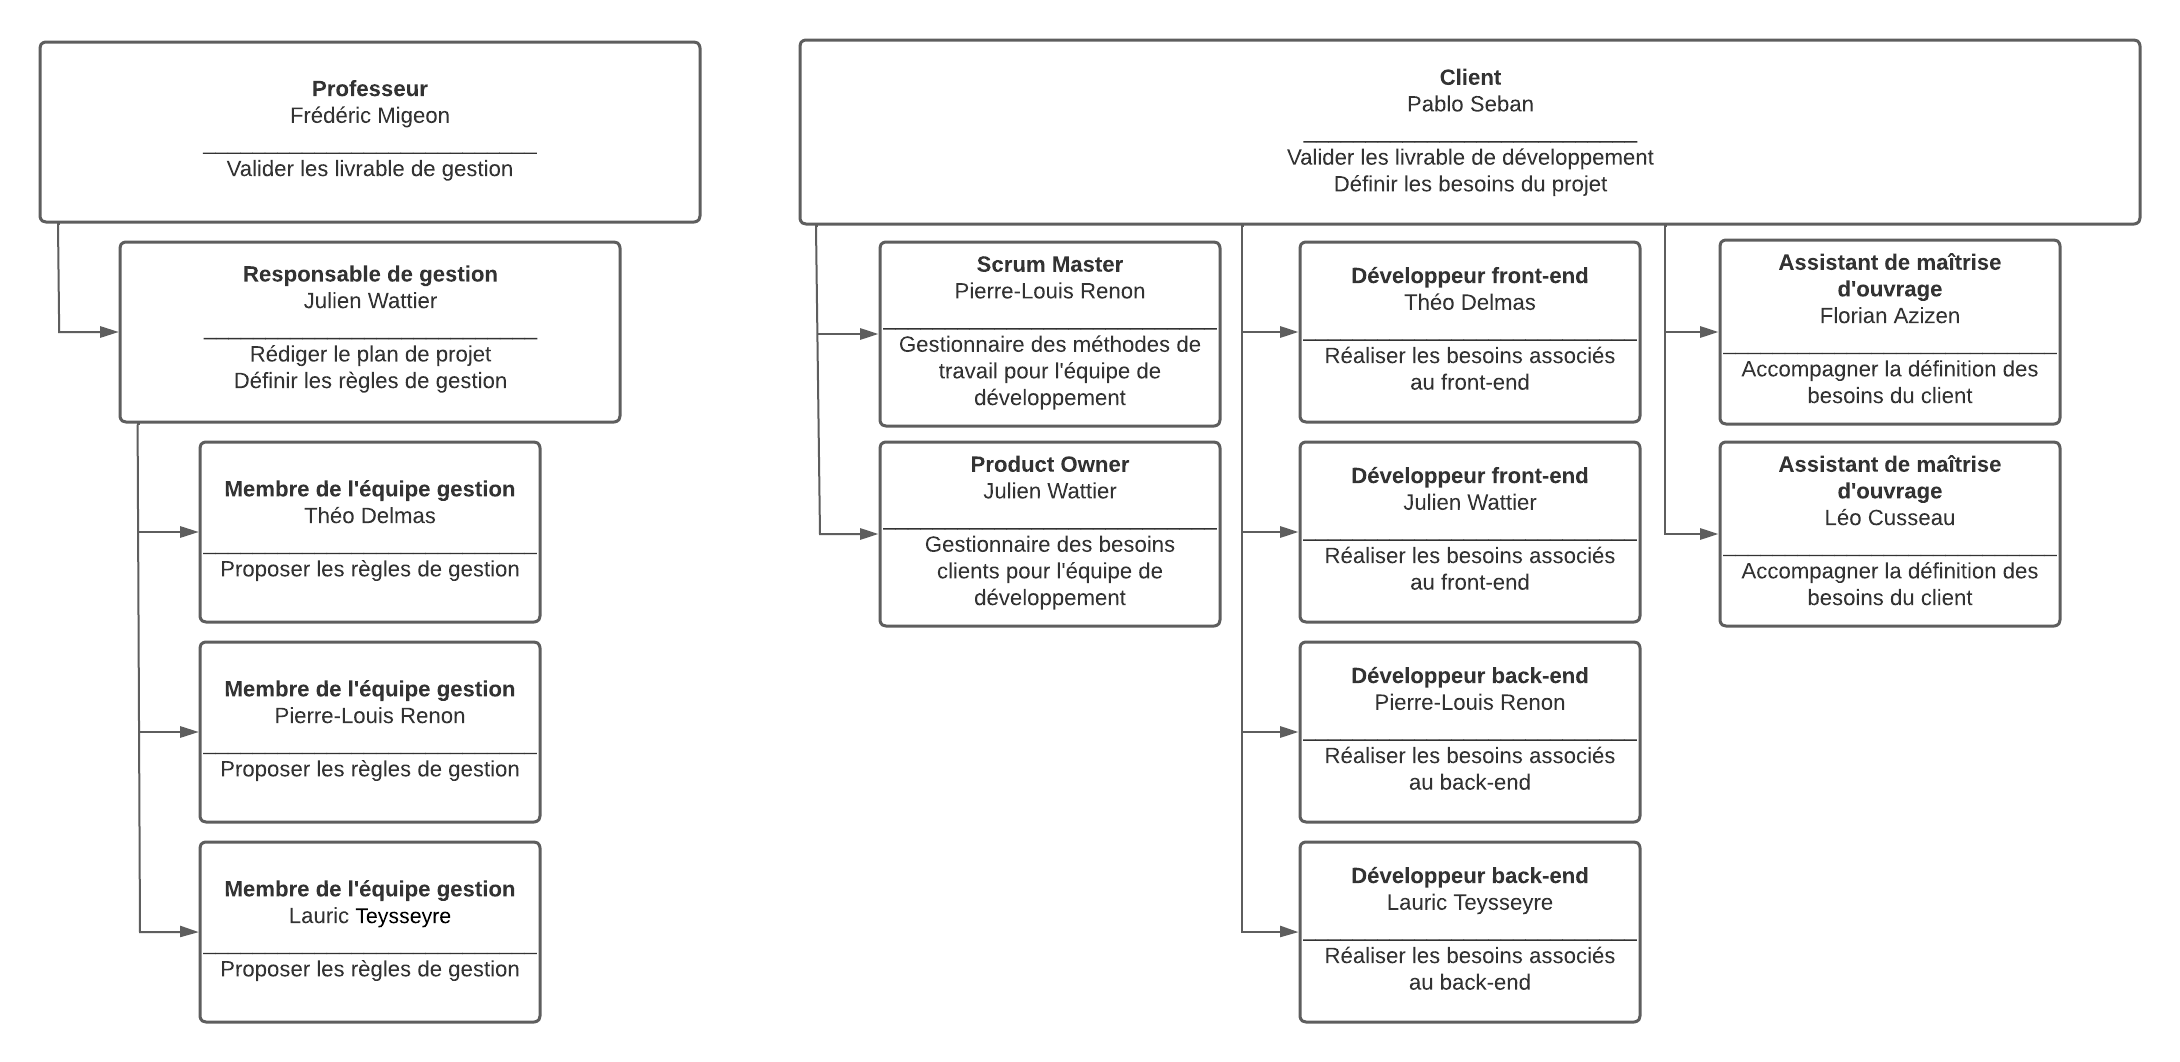
\includegraphics[scale=0.32]{documents/IMG/OBS}
         \end{subsubsection}

         \begin{subsubsection}{\label{sec:Matrice RACI}Matrice RACI}
             La matrice suivante définie les responsabilités de chaque activité pour chaque rôle. Cette responsabilité est défini selon la codification suivante :
             \begin{itemize}
                 \item[R]: Est responsable de la tâche.
                 \item[A] : Valide ou non la tâche lorsqu’elle est réalisée.
                 \item[C] : Contribue à la réalisation de la tâche.
                 \item[I] : Est informé des avancements et décisions relatives à la tâche.
             \end{itemize}
             \begin{landscape}
                 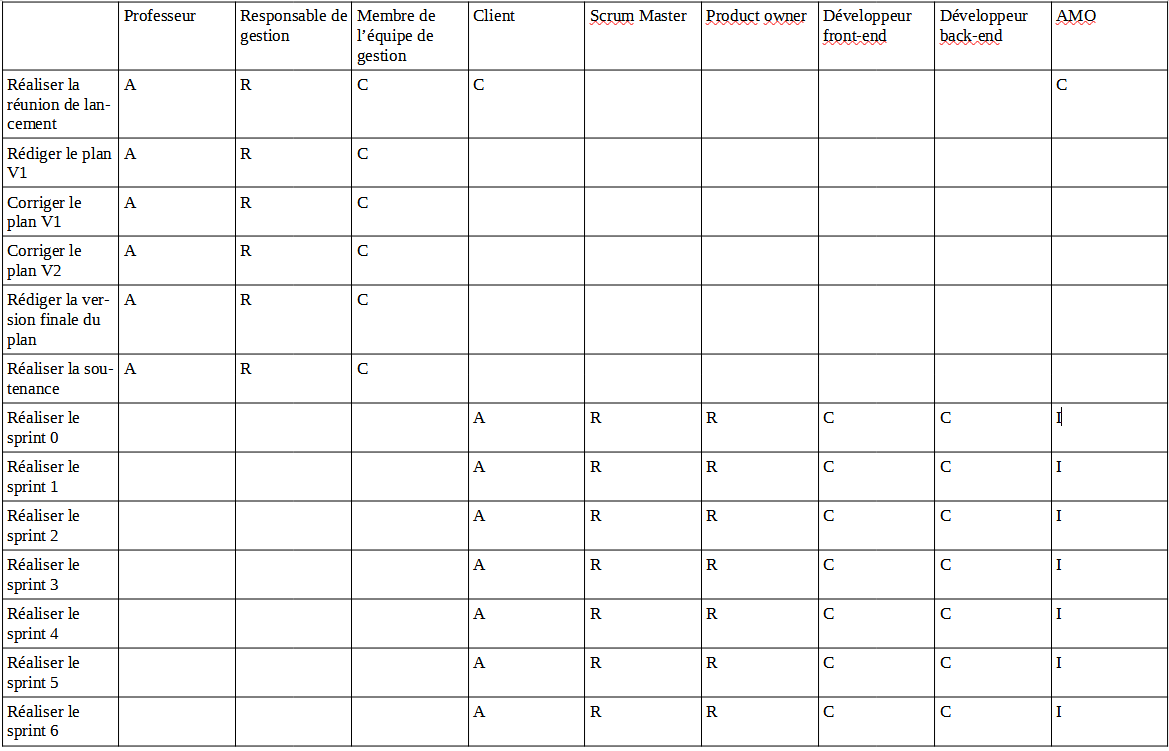
\includegraphics[scale=0.6]{documents/IMG/RACI}
             \end{landscape}
         \end{subsubsection}

     \end{subsection}

     \begin{subsection}{\label{sec:Suivi de déroulement}Suivi de déroulement}
         \begin{subsubsection}{\label{sec:Suivi du contexte}Suivi du contexte}
             //Faire un log de faits marquants par sprint.
         \end{subsubsection}

         \begin{subsubsection}{\label{sec:Gestion des décision}Gestion des décision}
             Les décisions relatives aux projet sont traçables dans le \href{documents/Registre_des_décisions.pdf}{registre des décisions}.

             Chaque décision y est décrite par sa description, qui précise ce qu’elle a modifié dans le plan projet, la justification/le contexte ayant nécessité cette décision ainsi que la date.

             Lorsqu’une décision est créée, le plan projet est alors actualisé conformément à la décision et mis à jour sur l’outil de gestion de version associé.
         \end{subsubsection}

         \begin{subsubsection}{\label{sec:Gestion des actions}Gestion des actions}
             Le suivi des actions à réaliser/réalisé est disponible sur le kanban (voir \hyperref[sec:Référencement des besoins]{le référencement des besoins}) grâce aux listes de tâches qu’il est possible d’associer à un besoin.
         \end{subsubsection}
     \end{subsection}

     \begin{subsection}{\label{sec:Gestion de la communication}Gestion de la communication}
         \begin{subsubsection}{\label{sec:Communication avec les parties prenantes}Communication avec les parties prenantes}
             Les communications avec les professeurs se feront de manière informelle lors de TD dédié à l’UE de projet.

             Pour les communications avec le client, elles se feront au travers du discord de FlOpEDT, que ce soit de manière textuelle pour des questions spontanée, ou vocale pour ce qui concerne les revues de sprint. Ces dernières se tenant dans les jours suivant la fin d’un sprint, fonction des disponibilités de chacun.

             Les revues de sprint seront enregistrées, puis traitées ultérieurement afin de produire un compte rendu de réunion référencé dans le \href{documents/Registre_des_rapports_de_réunion.pdf}{registre des rapports de réunion}. Ces rapports résument les retours du client afin que ces derniers soient référencés en tant qu’action ou décision à réaliser.

             Le reste des parties prenantes ne sera pas informé de l’avancée du projet, mais pourra le suivre via \href{https://github.com/Szyckaa/UE-PROJET-DOCS-GESTION}{ce dépôt distant} qui trace le plan de projet et les documents liés.
         \end{subsubsection}

         \newpage

         \begin{subsubsection}{\label{sec:Communication au sein de l'équipe}Communication au sein de l'équipe}
             L’équipe communique au travers d’un serveur discord dédié de manière informelle.

             Au début de chaque journée, une daily meeting informelle est organisée pour résumer le travail effectué par chacun lors de la dernière journée, les difficultés rencontrées et le travail prévu sur la journée.

             Par la suite les membres sont tous présents en vocal sur ce même serveur, et partage éventuellement leur écran afin de montrer ce qu’ils font.

             Enfin, pour faciliter le débugage, l’outil de peer-programming liveshare sera utilisé. Chaque développeur devra lancer une session de partage permettant aux autres membres d’avoir accès à leur code local.
         \end{subsubsection}
     \end{subsection}

     \begin{subsection}{\label{sec:Gestion de la qualité de management}Gestion de la qualité de management}
         \begin{subsubsection}{\label{sec:Qualité des produits}Qualité des produits}
            L'ensemble des documents seront produit en Latex.

             Les différentes versions du plan de projet sont revues par tous les membres de l’équipe avant soumission en tirant profit des fonctionnalités fournies par l'outil de gestion de version sur lequel ces documents sont suivis (voir la \hyperref[sec:Communication avec les parties prenantes]{gestion de la communication}).

             Chaque version du plan est également soumise à une évaluation interne grâce à une \href{Check_list.ods}{check-list} fournie par les professeurs. Cette liste conserve les réponses des anciennes versions afin d’évaluer l’évolution du plan.

             Enfin, chaque version est revue par les professeurs.
         \end{subsubsection}

         \begin{subsubsection}{\label{sec:Qualité des activités}Qualité des activités}
             L’équipe ne supervise pas les activités de management.
         \end{subsubsection}
     \end{subsection}

     \begin{subsection}{\label{sec:Gestion des risques et opportunités}Gestion des risques et opportunités}
         \begin{subsubsection}{\label{sec:Référencement des risques}Référencement des risques}
             La liste des risques et opportunités est listée dans le \href{documents/Registre_des_risques.pdf}{registre des risques et opportunités}.

             Chaque risque y est décrit par les champs suivants :
             \begin{itemize}
                 \item Titre du risque.
                 \item Description du risque.
                 \item Risque d’occurrence : sur une échelle faible - moyen - fort.
                 \item Niveau d'impact : sur une échelle fable - moyen - fort
                 \item Plan d'action : actions à mettre en place si le risque se déclenche ou est sur le point de se déclencher.
             \end{itemize}

             S'y ajoute les champs suivants si il y a déclenchement du risque :
             \begin{itemize}
                 \item Date de déclenchement.
                 \item Contexte de déclenchement.
             \end{itemize}
         \end{subsubsection}

         \begin{subsubsection}{\label{sec:Identification des risques}Identification des risques}
             Les risques ont été identifiés lors de l'élaboration de la note de cadrage.

             Si, lors de la capture d'un besoin, un risque apparaît comme évident aux fournisseurs, il sera ajouté dans le registre. Mais l'équipe ne dédiera pas particulièrement de temps à l'identification des risques.
         \end{subsubsection}

         \begin{subsubsection}{\label{sec:Réponse au risques}Réponse au risques}
             En cas de déclenchement d'un risque, l'équipe fournisseur suivra le plan d'action prévu dans le registre. Elle veillera également à remplir les champs associés au déclenchement dans le registre.

             Dans le cas de certains risques relativement génériques, l'équipe remplira plusieurs fois les champs de déclenchement.
         \end{subsubsection}
     \end{subsection}
    \end{section}

\newpage

    \begin{section}{\label{sec:Référentiel de développement de projet}Référentiel de développement de projet}
     L’équipe applique une méthode de développement hybride qui mixe le SCRUM et le kanban. Dans cette méthode, le travail est segmenté temporellement en sprint afin de ne pas perdre de vue le temps. Cependant elle gère les besoins en kanban. Il n’y a donc pas d’estimation de valeur des user stories pour savoir laquelle développer, ni d’objectif de durée pour réaliser un besoin.
     \begin{subsection}{\label{sec:Gestion des besoins}Gestion des besoins}
         \begin{subsubsection}{\label{sec:Référencement des besoins}Référencement des besoins}
             Les besoins sont suivis grâce à ce \href{https://wekan.flopedt.org/b/HsRkBw5rbmQt5PQet/catalogue}{kanban}. Celui-ci se décompose en deux parties. La première définit les principaux produits du projet et permet aux parties prenantes de comprendre sur quel produit l'équipe travaille actuellement. Les produits ayant été définis lors de la kick-off meeting.

             La seconde est un kanban lié au produit en cours. L'ensemble des besoins y sont retranscrits et décrits grâce à des user stories sur lesquelles l'équipe fournisseur adjoint une liste d'actions à effectuer afin de satisfaire la user story.

             Le kanban se divise en 5 colonnes :
             \begin{itemize}
                 \item Idée floue : La user story nécessite d'être raffinée en ajoutant les actions à effectuer qui y sont relatives. Cette colonne permet de noter informellement les besoins du clients.
                 \item À faire : La user story a été définie mais pas choisie pour le sprint en cours.
                 \item En cours : La user story a été choisie pour le sprint en cours.
                 \item A tester : La user story est satisfaite mais nécessite une validation via des tests unitaires et d’intégration, une approbation de la part du client, ainsi qu’une documentation du code source.
                 \item Ok : La user story a été testée et validée par le client.
             \end{itemize}

             Chaque user story est priorisée via sa position dans son couloir, et relativement aux besoins du client. Cette priorisation est définie par le client.

             Cet outil mixe donc le backlog ; puisqu’il référence les besoins ; et le kanaban ; puisque les tâches à effectuer sont ajoutés au sein de chaque besoin.

             Chaque développeur peut manipuler le kanban sans autorisation particulière.
         \end{subsubsection}


         \begin{subsubsection}{\label{sec:Définition de ready}Définition de ready}
            L'ensemble des critères suivants représentent la définition de ready des besoins traités ; c'est à dire que le besoin est passé en "A faire" (voir \hyperref[sec:Référencement des besoins]{référencement des besoins}) : 
            \begin{itemize}
                \item le besoin est décrit par une user story sous la forme "En tant <Catégorie d'utilisateur> je désire <fonctionnalité> afin de <intérêt de la fonctionnalité>.
                \item Une première liste d'action nécessaire pour réaliser ce besoin a été adjointe au besoin.
                \item Chaque développeur a approuvé la description textuelle et la liste d'action à effectuer.
            \end{itemize}
        \end{subsubsection}

        \begin{subsubsection}{\label{sec:Définition de done}Définition de done}
            L'ensemble des critères suivants représentent la définition de done des besoins traités ; c'est à dire que le besoin est passé en "OK" (voir \hyperref[sec:Référencement des besoins]{référencement des besoins}) : 
            \begin{itemize}
                \item le développement relatif au besoin est terminé.
                \item les règles de qualité développement sont respectées(voir la \hyperref[sec:Gestion de la qualité]{gestion de la qualité})
            \end{itemize}
        \end{subsubsection}

         \begin{subsubsection}{\label{sec:Capture des besoins}Capture des besoins}
             Une première partie des besoins a été capturé lors de la kick-off meeting et sa préparation.
             Les besoins sont capturés lors des revues de sprint en fonction des remarques du client sur ce qui est présenté. Lors de la production du rapport de revue (voir la \hyperref[sec:Gestion de la communication]{gestion des communications}) dans les jours suivants la réunion, les besoins sont alors raffinés et placés en à faire.

             Si un nouveau besoin fait apparaître un nouveau produit, alors une décision sera émise pour faire changer le référentiel.

             Le client défini la nouvelle priorité des besoins à réaliser à chaque sprint.
         \end{subsubsection}

         \begin{subsubsection}{\label{sec:Gestion des changement dans les besoins}Gestion des changement dans les besoins}
             Lors des revue de sprint le client à la possibilité d’émettre des remarques pouvant faire évoluer les besoins et tâches.

             Lors de la production du rapport de revue (voir la \hyperref[sec:Gestion de la communication]{gestion des communications}) dans les jours suivants la réunion, ces remarques sont alors transformées en actions et ajoutées sur le besoin associé.
         \end{subsubsection}
     \end{subsection}

     \begin{subsection}{\label{sec:Gestion du développement}Gestion du développement}
         Le développement suivra le workflow git. Il y aura donc une branche maîtresse intégrant les releases (artefact d’un sprint), une branche de développement intégrant les features en cours de développement et des branches de features correspondant au traitement d’un besoin.
     \end{subsection}

     \begin{subsection}{\label{sec:Gestion de la configuration}Gestion de la configuration}
         Les produits de ce projet seront tracés à l'aide de git, sur le \href{https://framagit.org/flopedt/FlOpEDT}{dépot officiel de FlopEDT}, et en particulier sur la branche \href{https://framagit.org/flopedt/FlOpEDT/-/tree/catalog}{catalog}.

         Chaque développeur dispose des droits et responsabilités sur les actions qu'il entreprend relativement à ce dépôt.
     \end{subsection}

     \begin{subsection}{\label{sec:Gestion des livrables}Gestion des livrables}
         \begin{subsubsection}{\label{sec:Processus de livraison}Processus de livraison}
             Lorsque les fonctionnalités seront considérées comme terminées elles seront intégrées dans la branche maîtresse, ce qui marquera la livraison au client.

             L’équipe s’assurera d’intégrer uniquement des fonctionnalités terminées donc fonctionnelles et testées.
         \end{subsubsection}

         \begin{subsubsection}{\label{sec:Suvi des livraisons}Suvi des livraisons}
             Le commit de merge dans la branche maîtresse (voir la \hyperref[sec:Gestion du développement]{gestion du développement}) permet de tracer les livrables livrés.
         \end{subsubsection}

         \begin{subsubsection}{\label{sec:Livraison finale}Livraison finale}
             Une revue de code sera organisée avec le client et des collaborateurs du projet au moment de la dernière livraison afin de faciliter la reprise du travail produit. La livraison final se fera selon les modalités classiques (voir le \hyperref[sec:Processus de livraison]{processus de livraison}).
         \end{subsubsection}
     \end{subsection}

     \begin{subsection}{\label{sec:Gestion de la qualité}Gestion de la qualité}
         \begin{subsubsection}{\label{sec:Front-end}Front-end}
             Le code produit est soumis à l’outil de vérification ESLint, ce qui permet d’avoir une syntaxe homogène mais également d’optimiser le code en appliquant des bonnes pratiques qui sont vérifiées par l’outil.

             Le code est documenté en ajoutant de la JSDoc à chaque méthode, variable et classe et en tirant profit des annotations offert par la JSDoc. Concernant les composants, ils sont documentés à l’aide d’un entête au début de la section de script qui récapitule ce que fait le composant. Après cet entête se trouve les props documentés du composant, puis les emits documentés. Ainsi l’ensemble de l’interface du composant est localisé au même endroit et est documenté.
         \end{subsubsection}

         \begin{subsubsection}{\label{sec:Back-end}Back-end}
             L’essentiel des développements back-end consiste à produire des API utilisées par le front-end. Ces API seront développées selon la convention RESTFull.

             Le code est documenté en ajoutant de la documentation à chaque méthode, variable et classe.
         \end{subsubsection}

         \begin{subsubsection}{\label{sec:Revue de code}Revue de code}
             L’équipe tire profit des fonctionnalités de l’outil de gestion de version (voir la \hyperref[sec:Gestion de la configuration]{gestion de la configuration}) en imposant une revue de code avant d’intégrer une fonctionnalité dans la branche de développement. L’intégration doit être validée par au moins deux développeurs différents de celui qui a développé la fonctionnalité.
         \end{subsubsection}

         \begin{subsubsection}{\label{sec:Revue de sprint}Revue de sprint}
             Les revues de sprint permettent la validation oral du client sur un besoin, afin de savoir si la réalisation de ce dernier par l’équipe de développement corresponds bien à ces attentes.
         \end{subsubsection}
     \end{subsection}
    \end{section}

    \begin{section}{\label{sec:Bilan de projet}Bilan de projet}
     \begin{subsection}{\label{sec:Référencement du bilan}}
         Le bilan est référencé dans le \href{documents/Bilan_de_projet.pdf}{document dédié}.
     \end{subsection}

     \begin{subsection}{\label{sec:Production du bilan}}
         Le bilan sera produire après livraison du la dernière version du plan projet.
         Ce dernier, ainsi que le documents évolutifs mis à jour relativement aux derniers événement du projet seront disponibles au travers d’une release sur l’outil de gestion de version qui trace les documents de gestion (voir la \hyperref[sec:Communication avec les parties prenantes]{communication avec les parties prenantes}).
     \end{subsection}
    \end{section}
}

\end{document}

%     \label{test}
% \hyperref[test]{goto} se base sur quelques principes simples de relations causales... etc.